\subsection{Shape}

During the development phase, we began translating the conceptual design of the robot into a tangible and expressive physical form. The original inspiration was a cooking pot—round, friendly, and slightly whimsical—symbolizing the robot's function related to managing microwave access. However, as construction progressed, we adapted this concept to fit the realities of available tools, materials, and structural constraints in the lab.

As previously mentioned, the robot's physical skeleton was built using \textbf{two dodecagonal wooden platforms}—a base and a top—offering a structure that approximates a circular form while being much easier to manufacture using flat wood sheets. This polygonal configuration provided excellent stability, allowed consistent mounting points, and gave us an ideal layout for placing the ultrasonic sensors around the perimeter, on alternating sides.

Once the structural base was completed and tested, we began the \textbf{aesthetic transformation} of the robot. In the first stage the robot was covered with a \textbf{white fabric draped over the wooden base}, giving it a soft and continuous outer surface. At this point, we also added the \textbf{first vertical supports} that would later hold the turn-dispenser module, made of transparent tubing and filled with balls to simulate a ticket lottery system.

\begin{figure}[H]
    \centering
    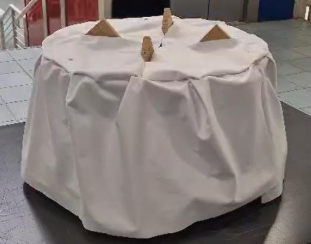
\includegraphics[width=0.6\linewidth]{../ReportMovementModule/images/Aspose.Words.728084da-df58-4b9d-a372-f65cffbdb23d.026.png}
    \caption{Initial Fabric Cover}
\end{figure}

In the second stage, we moved beyond the clean fabric and began attaching \textbf{cotton padding} all around the robot. This gave the robot a fluffy, cloud-like appearance, softening its visual presence and introducing a playful, imaginative look that would appeal to users. This cotton layer also served to subtly obscure the structural hardware beneath, enhancing the illusion of a light, floating device.

\begin{figure}[H]
    \centering
    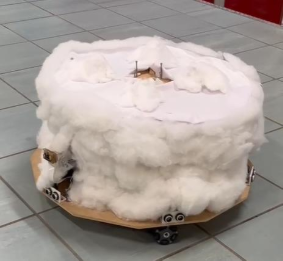
\includegraphics[width=0.6\linewidth]{../ReportMovementModule/images/Aspose.Words.728084da-df58-4b9d-a372-f65cffbdb23d.027.png}
    \caption{Cloud-like Cotton Layer}
\end{figure}

Finally we embedded \textbf{LED lights inside the cotton structure}, creating a visual effect reminiscent of a \textbf{storm cloud}. When lit from within, the cotton shimmered and pulsed, adding depth and dynamic texture to the robot's presence. This stage brought the design much closer to an animated, expressive character rather than just a mobile object.

\begin{figure}[H]
    \centering
    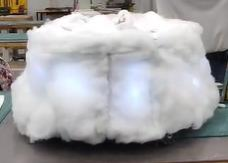
\includegraphics[width=0.6\linewidth]{../ReportMovementModule/images/Aspose.Words.728084da-df58-4b9d-a372-f65cffbdb23d.028.png}
    \caption{LED-Enhanced Cloud Appearance}
\end{figure}

Throughout this process, we continuously adjusted the shape based on technical needs and visual testing. The final form successfully merges functionality and storytelling, transforming the movement module from a structural base into a \textbf{key part of a characterful robot}.
